%! Author = kyoto
%! Date = 08.03.2022


\section{Задание}
По выданному преподавателем варианту разработать программу асинхронного обмена данными с внешним устройством. При помощи
программы осуществить ввод или вывод информации, используя в качестве подтверждения данных сигнал (кнопку) готовности ВУ.


\begin{figure}[H]
    \centering
    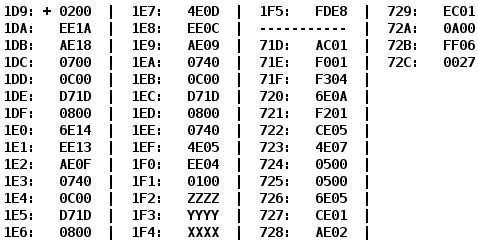
\includegraphics[scale=0.35]{img/variant}
\end{figure}


\section{Программа}

\subsection{Assembler}

\begin{center}
    \begin{tabular}{c}
        \begin{lstlisting}[basicstyle=\ttfamily]
        ORG     0x360
ADDR:	WORD	0x5A1
LEN:	WORD	0x0000
FIRST:	WORD	0x0000
SECOND: WORD    0x0000
START:  LD      (ADDR)+
        AND     #0xFF
        ST      LEN
L:      IN      7
        AND     #0x40
        BEQ     L
        LD      LEN
        OUT     6
BEGIN:	CLA
        LD      (ADDR)+
        ST      FIRST
        SWAB
        ST      SECOND
S1:     IN      7
        AND     #0x40
        BEQ     S1
        LD      FIRST
        OUT     6
        LOOP    LEN
        JUMP    S2
        JUMP    STOP
S2:     IN      7
        AND     #0x40
        BEQ     S2
        LD      SECOND
        OUT     6
        LOOP    LEN
        JUMP    BEGIN
STOP:	HLT

        \end{lstlisting}
    \end{tabular}
\end{center}

\newpage

\subsection{Основная:}

\subsection{Описание программы:}
Вывод текста сохранённого в массиве в формате АДР0: ДЛИНА АДР1: СИМВ2 СИМВ1 АДР2: СИМВ4 СИМВ3 ... \\
\footnotesize (выводит сначала количество символов, а потом символы в порядке возрастания: СИМВ1, СИМВ2, СИМВ3)\\
\normalsize


\section{Область представления данных и область допустимых значений}

\subsection{Область представления:}
\noindentВ ячейке 360 беззнаковое 11тиразрядное 16теричное число (адрес ячейки).   \\
В ячейках 362-363 символ строки в кодировке ISO-8859-5. \\
В ячейке 361, 5A1 беззнаковое 8миразрядное 16теричное число.    \\
В дальнейших ячейках массива - беззнаковые 16теричные числа, с закодированными символами в младшем и старшем байте. \\

\newpage

\subsection{ОДЗ}

\subsubsection{ADDR:}
\begin{equation*}
    \begin{center}
        $0_{16} \leqslant ADDR \leqslant 7FF_{16}$\\
    \end{center}
\end{equation*}

\subsubsection{LEN:}
\begin{equation*}
    \begin{center}
        $0_{16} \leqslant LEN \leqslant FF_{16}$\\
        (на самом деле там одз нет, потому что мы выделяем маской значащие биты)
    \end{center}
\end{equation*}

\subsubsection{$M_i$:}
\begin{equation*}
    \begin{center}
        $20_{16} \leqslant $M_{i}$ \leqslant FF_{16}$\\
        (имеется ввиду ограничение на младший и старший байт элементов массива)
    \end{center}
\end{equation*}


\section{Расположение программы в памяти БЭВМ:}
\noindent\textit{Программы - \textbf{360-380} . \\
Выводимая строка – \textbf{5A1-(5A1+LEN-1)} .  \\}


\newpage


\section{Исполнение.}

\subsection{Выводимая строка:}
\begin{center}
    \begin{tabular}{|c|c|c|c|}
        \hline
        \textbf{Symbol} & \textbf{ISO-8859-5} & \textbf{UTF-8} & \textbf{UTF-16} \\
        \hline
        В               & 0xB2                & 0xD092         & ?               \\
        Е               & 0xB5                & 0xD095         & ?               \\
        Т               & 0xC2                & 0xD0A2         & ?               \\
        В               & 0xB2                & 0xD092         & ?               \\
        Ь               & 0xCC                & 0xD0AC         & ?               \\
        \hline


    \end{tabular}
\end{center}
